\documentclass{beamer}

\usepackage[utf8]{inputenc}
\usepackage[russian]{babel}
\usepackage{default}

\usepackage[scaled]{DejaVuSansMono}

\setbeamertemplate{footline}[frame number]
\setbeamertemplate{navigation symbols}{}
\setbeamertemplate{blocks}[rounded][shadow=true]
\setbeamercolor{block title}{use=structure,fg=white,bg=blue!75!black}
\beamertemplateballitem

\mode<presentation>{
  \usetheme{default}
}

\theoremstyle{definition}
% coloring tables
\usepackage{hhline}
\usepackage{colortbl}
\usepackage{xcolor}
\definecolor{YellowGreen} {HTML}{B5C28C}
\definecolor{ForestGreen} {HTML}{009B55}
\definecolor{Blueish}{HTML}{A6C5E1}
\newcommand{\RowColor}{\rowcolor{red!50} \cellcolor{white}}

%% colored links
% \definecolor{links}{HTML}{2A1B81}
\hypersetup{colorlinks,linkbordercolor=red,linkcolor=,urlcolor=blue}
% \hypersetup{colorlinks=true,linkbordercolor=red,urlcolor=blue,pdfborderstyle={/S/U/W 1}}
\usepackage{hyperref}          % clickable URls and cross-references
%%%% code listings
\usepackage{minted}

\usepackage{fontawesome}
\newcommand{\faGood}{\textcolor{ForestGreen}{\faThumbsUp}}
\newcommand{\faBad}{\textcolor{red}{\faThumbsODown}}
%fancy letters
\newcommand{\jsoo}{Js\_of\_ocaml }
\usepackage{mathrsfs,amsmath}
\usepackage{mathtools}  % for xRightArrow
\usepackage{tikz}

\newcommand{\trollface}{\resizebox{\fontcharht\font`X}{\fontcharwd\font`X}{%
\begin{tikzpicture}[y=0.80pt, x=0.8pt,yscale=-1, inner sep=0pt, outer sep=0pt]
\path[fill=black,even odd rule] (186.5230,42.6290) .. controls
  (181.3770,46.8210) and (177.2520,52.0360) .. (177.1840,61.3090) .. controls
  (173.4610,53.8470) and (177.9210,43.3950) .. (186.5230,42.6290) -- cycle;
\path[fill=black,even odd rule] (123.9480,53.8360) .. controls
  (131.6610,49.6690) and (133.9770,68.5560) .. (129.5520,73.4490) .. controls
  (130.1610,64.4350) and (129.6880,56.5020) .. (123.9480,53.8360) -- cycle;
\path[fill=black,even odd rule] (258.4390,84.6570) .. controls
  (251.9670,92.1160) and (243.0990,85.7280) .. (234.1560,84.6570) .. controls
  (214.8650,82.3460) and (196.3430,90.9360) .. (182.7880,96.7990) .. controls
  (152.3050,81.2930) and (190.8780,59.8650) .. (221.0810,61.3090) .. controls
  (241.5710,62.2870) and (255.3680,71.4410) .. (258.4390,84.6570) --
  cycle(206.1380,68.7800) .. controls (196.6960,73.9690) and (181.3370,73.2430)
  .. (180.9200,87.4590) .. controls (194.1550,88.2420) and (196.7990,78.4330) ..
  (209.8730,79.0540) .. controls (208.5950,75.6620) and (209.3090,70.2780) ..
  (206.1380,68.7800) -- cycle(249.1000,80.9220) .. controls (248.1190,76.6100)
  and (244.5910,74.8460) .. (238.8270,75.3180) .. controls (238.2690,81.1680)
  and (246.1370,78.5920) .. (249.1000,80.9220) -- cycle;
\path[fill=black,even odd rule] (135.1560,84.6570) .. controls
  (139.6320,83.6130) and (143.7260,82.0440) .. (147.2980,84.6570) .. controls
  (147.0140,91.5340) and (139.4010,91.0810) .. (135.1560,93.9970) .. controls
  (135.1560,99.9120) and (135.1560,105.8270) .. (135.1560,111.7420) .. controls
  (129.8970,116.4450) and (122.1800,118.6910) .. (118.3440,124.8180) .. controls
  (121.4790,132.8890) and (127.0330,138.5440) .. (134.2210,142.5630) .. controls
  (138.8510,142.3020) and (140.5480,137.0180) .. (145.4290,139.7610) .. controls
  (138.6120,162.3790) and (120.0140,140.4880) .. (112.7400,131.3550) .. controls
  (110.2100,132.5610) and (109.4200,135.5060) .. (105.2680,135.0910) .. controls
  (105.7160,132.1530) and (103.9380,131.4400) .. (103.4000,129.4870) .. controls
  (96.0960,131.2120) and (93.0790,137.2230) .. (83.7870,136.9590) .. controls
  (100.7200,129.2980) and (112.9440,116.9280) .. (127.6830,107.0720) .. controls
  (127.6830,102.7140) and (127.6830,98.3550) .. (127.6830,93.9970) .. controls
  (115.4770,85.0330) and (89.1830,90.1570) .. (75.3810,82.7890) .. controls
  (83.6980,60.8440) and (125.4950,70.6300) .. (135.1560,84.6570) --
  cycle(88.4580,79.0540) .. controls (93.0320,80.8510) and (100.4610,79.8720) ..
  (104.3350,78.1190) .. controls (99.7600,76.3220) and (92.3310,77.3020) ..
  (88.4580,79.0540) -- cycle;
\path[fill=black,even odd rule] (262.1750,78.1190) .. controls
  (266.1280,76.3740) and (271.8460,80.8820) .. (278.0530,79.9870) .. controls
  (278.0700,84.9570) and (269.8980,85.7630) .. (265.9110,83.7230) .. controls
  (266.0380,81.0470) and (272.3220,84.5300) .. (272.4490,81.8550) .. controls
  (269.2020,80.4330) and (264.6140,80.3510) .. (262.1750,78.1190) -- cycle;
\path[fill=black,even odd rule] (71.6460,81.8550) .. controls
  (48.4920,80.0360) and (22.9120,89.3230) .. (22.1460,111.7420) .. controls
  (22.0350,114.9910) and (22.2010,122.2410) .. (24.9480,126.6850) .. controls
  (29.3060,133.7360) and (40.2990,130.2490) .. (43.6270,139.7610) .. controls
  (26.4310,135.6320) and (18.5280,125.8960) .. (20.2780,108.9400) .. controls
  (22.7070,85.3990) and (45.7110,76.5680) .. (71.6460,81.8550) -- cycle;
\path[fill=black,even odd rule] (335.0240,98.6670) .. controls
  (328.5190,86.1820) and (314.4580,81.2520) .. (293.9290,82.7890) .. controls
  (309.8870,79.1500) and (332.2580,83.1200) .. (335.0240,98.6670) -- cycle;
\path[fill=black,even odd rule] (262.1750,87.4590) .. controls
  (263.4210,84.8030) and (266.3280,88.1800) .. (267.7790,88.3940) .. controls
  (266.4780,91.1060) and (263.1700,88.1290) .. (262.1750,87.4590) -- cycle;
\path[fill=black,even odd rule] (219.2130,88.3940) .. controls
  (228.9990,89.9850) and (233.5670,100.3980) .. (245.3640,101.4690) .. controls
  (259.7920,102.7790) and (267.3080,92.6370) .. (279.9210,89.3270) .. controls
  (314.2440,80.3190) and (342.0750,112.2860) .. (316.3460,139.7620) .. controls
  (312.1960,130.4970) and (320.4280,125.8410) .. (319.1480,114.5440) .. controls
  (317.6560,101.3880) and (305.0200,92.5910) .. (290.1950,94.9310) .. controls
  (285.2060,95.7190) and (280.8230,101.1010) .. (275.2520,103.3370) .. controls
  (255.1770,111.3950) and (219.5950,110.7840) .. (219.2130,88.3940) -- cycle;
\path[fill=black,even odd rule] (45.4950,90.2610) .. controls
  (42.3020,96.1040) and (28.5930,99.5050) .. (33.3530,116.4120) .. controls
  (28.6240,112.2490) and (33.6510,103.5000) .. (32.4190,96.7990) .. controls
  (36.9290,94.7710) and (41.1020,92.4060) .. (45.4950,90.2610) -- cycle;
\path[fill=black,even odd rule] (84.7220,108.0070) .. controls
  (88.8510,106.8440) and (89.8150,102.5150) .. (95.9300,103.3370) .. controls
  (99.8760,115.4730) and (84.1750,115.7950) .. (72.5810,115.4790) .. controls
  (71.5810,110.8750) and (69.6390,107.2120) .. (66.0430,105.2050) .. controls
  (55.3470,104.1610) and (49.0010,107.4650) .. (39.8920,108.0080) .. controls
  (44.8020,88.7320) and (76.0790,99.0260) .. (84.7220,108.0070) -- cycle;
\path[fill=black,even odd rule] (313.5430,127.6200) .. controls
  (308.5690,129.4390) and (304.6380,127.2380) .. (299.5340,126.6850) .. controls
  (296.2380,129.2760) and (293.4220,135.3040) .. (295.7980,140.6950) .. controls
  (283.8630,150.9330) and (275.9310,169.7570) .. (264.0430,182.7230) .. controls
  (234.6970,214.7360) and (183.6470,228.5980) .. (117.4100,225.6860) .. controls
  (95.9890,224.7450) and (71.0460,222.4130) .. (60.4380,211.6760) .. controls
  (43.6320,194.6670) and (42.8320,141.9400) .. (57.6360,121.0810) .. controls
  (59.0730,118.1590) and (57.2280,111.9560) .. (60.4380,110.8080) .. controls
  (67.8970,113.3780) and (63.8270,124.2490) .. (66.0420,130.4210) .. controls
  (70.6570,143.2850) and (96.3870,151.5800) .. (114.6080,153.7710) .. controls
  (182.9370,161.9820) and (240.6520,126.1850) .. (285.5240,110.8080) .. controls
  (286.8670,107.4810) and (286.4780,102.4220) .. (289.2600,100.5350) .. controls
  (294.8400,102.4830) and (292.5530,107.1600) .. (294.8640,110.8080) .. controls
  (299.9820,118.8930) and (312.2430,119.4850) .. (313.5430,127.6200) --
  cycle(256.5710,133.2240) .. controls (256.5710,137.8940) and
  (256.5710,142.5640) .. (256.5710,147.2340) .. controls (274.1010,144.2160) and
  (289.2540,138.8220) .. (290.1940,119.2140) .. controls (274.7910,119.6880) and
  (268.9450,129.7200) .. (256.5710,133.2240) -- cycle(57.6360,143.4970) ..
  controls (59.9280,143.2360) and (61.9410,137.9240) .. (60.4380,136.9590) ..
  controls (59.6630,139.2970) and (57.8790,140.6280) .. (57.6360,143.4970) --
  cycle(205.2030,149.1020) .. controls (205.1680,155.3640) and
  (207.5990,159.1590) .. (208.0050,164.9790) .. controls (223.7610,158.0080) and
  (247.7210,159.2420) .. (249.1000,137.8940) .. controls (235.1800,138.6090) and
  (220.1700,146.3200) .. (205.2030,149.1020) -- cycle(66.9760,166.8470) ..
  controls (67.8590,159.9310) and (72.0280,150.7120) .. (67.9100,144.4320) ..
  controls (64.8520,149.0080) and (57.2650,163.7120) .. (66.9760,166.8470) --
  cycle(257.5050,174.3180) .. controls (259.8780,172.3290) and
  (263.2370,170.8490) .. (265.9110,167.7800) .. controls (269.5100,163.6490) and
  (276.6900,150.9880) .. (275.2510,150.9680) .. controls (264.4210,152.7880) and
  (248.8670,162.0370) .. (257.5050,174.3180) -- cycle(77.2500,170.5820) ..
  controls (81.8400,169.1510) and (85.3880,173.5910) .. (87.5240,171.5170) ..
  controls (84.1720,165.9570) and (90.7970,162.3580) .. (90.3260,156.5740) ..
  controls (84.8320,156.4640) and (82.4630,153.2290) .. (78.1840,151.9040) ..
  controls (73.1060,155.9740) and (76.7130,164.2210) .. (77.2500,170.5820) --
  cycle(195.8630,152.8370) .. controls (184.6230,155.6070) and
  (172.2560,157.2490) .. (161.3060,160.3090) .. controls (161.3060,164.9790) and
  (161.3060,169.6490) .. (161.3060,174.3190) .. controls (177.4140,175.4840) and
  (188.1850,171.3110) .. (200.5330,168.7150) .. controls (199.4780,162.9210) and
  (199.4950,156.0550) .. (195.8630,152.8370) -- cycle(94.0610,171.5170) ..
  controls (102.0880,173.7640) and (111.3050,174.8210) .. (122.0800,174.3190) ..
  controls (121.4640,169.8440) and (123.0400,164.0500) .. (122.0800,162.1770) ..
  controls (113.6500,161.2670) and (103.9510,161.6260) .. (97.7970,158.4420) ..
  controls (96.5510,162.7990) and (96.3510,168.2020) .. (94.0610,171.5170) --
  cycle(131.4200,162.1770) .. controls (131.6440,167.0710) and
  (129.1470,169.2430) .. (128.6180,173.3850) .. controls (135.5560,175.4760) and
  (146.2990,173.7610) .. (154.7690,174.3190) .. controls (154.7690,169.6490) and
  (154.7690,164.9790) .. (154.7690,160.3090) .. controls (145.9280,159.8740) and
  (140.7430,163.0940) .. (131.4200,162.1770) -- cycle(211.7410,178.0550) ..
  controls (210.4210,189.9590) and (217.7640,193.2010) .. (219.2130,202.3380) ..
  controls (232.4160,197.1720) and (241.9620,188.3510) .. (252.8360,180.8570) ..
  controls (247.5230,178.3850) and (247.9630,170.1630) .. (246.2980,164.0450) ..
  controls (236.3020,170.2380) and (224.6830,174.8070) .. (211.7410,178.0550) --
  cycle(168.7780,190.1960) .. controls (168.0510,199.3280) and
  (170.0950,205.6890) .. (169.7120,214.4780) .. controls (187.7230,215.6780) and
  (199.0090,210.1530) .. (211.7410,206.0730) .. controls (209.4850,196.8090) and
  (203.6060,191.1700) .. (203.3350,179.9220) .. controls (193.1930,184.7240) and
  (182.5080,188.9810) .. (168.7780,190.1960) -- cycle(66.0420,203.2710) ..
  controls (65.9030,195.9380) and (62.2210,192.1490) .. (58.5700,188.3280) ..
  controls (60.1730,194.1960) and (62.3150,199.5260) .. (66.0420,203.2710) --
  cycle(83.7880,211.6770) .. controls (81.6570,203.8460) and (79.4550,196.0850)
  .. (72.5800,192.9980) .. controls (72.0370,198.2100) and (75.3710,199.5460) ..
  (75.3820,204.2050) .. controls (74.8020,207.4170) and (70.3580,206.0980) ..
  (69.7780,207.0070) .. controls (73.0720,209.9390) and (78.5480,210.6890) ..
  (83.7880,211.6770) -- cycle(133.2880,195.8000) .. controls (133.3440,203.8380)
  and (136.3930,208.8840) .. (136.0900,217.2810) .. controls (144.8000,216.9630)
  and (154.9630,218.0960) .. (162.2410,216.3460) .. controls (161.9570,212.0840)
  and (160.6930,201.2210) .. (161.3070,192.9970) .. controls (152.8320,194.8520)
  and (141.9890,197.0030) .. (133.2880,195.8000) -- cycle(92.1930,212.6110) ..
  controls (95.7960,213.9890) and (99.2500,215.5160) .. (104.3350,215.4130) ..
  controls (103.0850,209.1910) and (98.9260,205.8780) .. (98.7310,198.6010) ..
  controls (93.8100,198.5410) and (91.8760,195.4940) .. (86.5890,195.7990) ..
  controls (87.4560,202.1920) and (94.9240,205.5740) .. (92.1930,212.6110) --
  cycle(106.2030,197.6680) .. controls (107.8940,204.6930) and
  (112.1030,209.2020) .. (113.6750,216.3470) .. controls (118.0900,216.6280) and
  (125.5740,218.7360) .. (129.5520,216.3470) .. controls (128.6800,203.5710) and
  (121.5510,192.9510) .. (106.2030,197.6680) -- cycle;
\path[fill=black,even odd rule] (197.7310,121.0820) .. controls
  (198.7120,132.7370) and (196.2330,144.5570) .. (184.6560,140.6950) .. controls
  (183.4110,132.5700) and (193.0760,132.9910) .. (191.1930,126.6850) .. controls
  (189.4350,120.7980) and (181.5510,124.0340) .. (174.3820,121.0810) .. controls
  (176.0420,109.8510) and (193.8450,115.8040) .. (197.7310,121.0820) -- cycle;
\path[fill=black,even odd rule] (200.5330,115.4790) .. controls
  (204.4700,115.3180) and (201.1740,117.5700) .. (200.5330,118.2810) .. controls
  (203.9060,128.7760) and (224.3770,116.4100) .. (228.5530,125.7530) .. controls
  (220.2110,119.9870) and (196.2170,130.8070) .. (200.5330,115.4790) -- cycle;
\path[fill=black,even odd rule] (31.4850,117.3460) .. controls
  (35.1880,120.4920) and (37.8990,124.6310) .. (42.6930,126.6860) .. controls
  (37.0450,129.1980) and (31.9330,123.1410) .. (31.4850,117.3460) -- cycle;
\path[fill=black,even odd rule] (180.9200,129.4870) .. controls
  (180.7300,132.4100) and (181.5500,136.3430) .. (179.9860,137.8930) .. controls
  (174.0290,133.1600) and (163.2140,138.0600) .. (154.7690,135.0910) .. controls
  (155.7830,124.9850) and (172.8760,127.2090) .. (180.9200,129.4870) -- cycle;
\path[fill=black,even odd rule] (258.4390,207.0070) .. controls
  (259.6460,209.1990) and (251.8250,210.0340) .. (248.1660,211.6770) .. controls
  (221.0230,223.8620) and (191.6300,245.8770) .. (151.0330,242.4980) .. controls
  (197.2180,241.0510) and (221.2870,217.4870) .. (258.4390,207.0070) -- cycle;
\path[fill=black,even odd rule] (65.1080,225.6870) .. controls
  (74.4620,238.4370) and (92.9790,242.0240) .. (113.6740,243.4320) .. controls
  (93.8120,244.9240) and (68.5880,243.6900) .. (65.1080,225.6870) -- cycle;
\path[fill=black,even odd rule] (161.3070,232.2250) .. controls
  (147.9730,232.8420) and (127.4930,235.8070) .. (112.7410,233.1590) .. controls
  (113.5640,233.3060) and (107.4200,234.1800) .. (110.8730,232.2250) .. controls
  (128.2930,233.0280) and (146.3320,230.9210) .. (161.3070,232.2250) -- cycle;
\path[fill=black,even odd rule] (127.6840,243.4320) .. controls
  (131.1270,241.2720) and (138.5660,243.1070) .. (143.5610,242.4980) .. controls
  (140.1180,244.6580) and (132.6790,242.8230) .. (127.6840,243.4320) -- cycle;
\path[fill=black,even odd rule] (38.0230,42.6290) .. controls (82.5390,0.2510)
  and (168.4500,6.1510) .. (250.9680,7.1380) .. controls (258.8160,7.2320) and
  (267.6870,5.7700) .. (274.3170,7.1380) .. controls (286.1880,9.5890) and
  (299.5410,24.1610) .. (306.0720,35.1580) .. controls (310.9170,43.3120) and
  (313.1390,55.1730) .. (317.2800,62.2430) .. controls (330.3650,84.5890) and
  (363.7570,90.1510) .. (354.6380,129.4880) .. controls (350.3990,147.7790) and
  (330.9450,155.1810) .. (321.0150,173.3850) .. controls (317.4380,179.9440) and
  (316.7720,187.3410) .. (313.5430,192.9980) .. controls (301.1180,214.7730) and
  (268.7750,231.0160) .. (241.6280,243.4320) .. controls (220.9940,252.8700) and
  (198.3130,267.1020) .. (179.0520,272.3850) .. controls (166.3570,275.8670) and
  (147.5010,278.7970) .. (128.6170,282.6580) .. controls (101.5110,288.2020) and
  (70.6950,290.9440) .. (49.2300,281.7240) .. controls (38.0840,276.9370) and
  (25.4570,265.4370) .. (23.0790,254.6390) .. controls (17.5010,229.3100) and
  (34.1810,186.6860) .. (26.8150,156.5730) .. controls (21.7590,135.9030) and
  (3.9090,121.6480) .. (10.0030,95.8650) .. controls (15.1720,74.0010) and
  (40.4630,75.0640) .. (38.0230,42.6290) -- cycle(346.2320,130.4220) .. controls
  (356.6420,101.6040) and (332.1320,76.8320) .. (298.5990,78.1190) .. controls
  (304.7890,76.0110) and (311.4390,78.0850) .. (318.2120,78.1190) .. controls
  (301.9840,58.2020) and (298.0540,17.1590) .. (264.0420,13.6760) .. controls
  (216.9920,8.8570) and (155.8050,15.1380) .. (110.8720,19.2800) .. controls
  (142.1830,27.4840) and (175.9850,13.4080) .. (208.9390,16.4780) .. controls
  (239.3500,19.3120) and (260.6870,37.8100) .. (277.1190,51.9690) .. controls
  (257.8750,41.2170) and (237.7900,21.1210) .. (208.0050,18.3460) .. controls
  (183.2390,16.0380) and (165.7270,22.7740) .. (144.4950,23.9500) .. controls
  (127.4810,24.8920) and (109.8000,20.5540) .. (94.9950,22.0820) .. controls
  (77.6030,23.8780) and (47.9860,38.7270) .. (43.6270,51.9700) .. controls
  (42.0390,56.7930) and (43.7690,62.7160) .. (41.7590,67.8470) .. controls
  (34.6190,86.0780) and (9.3930,91.1260) .. (18.4100,122.0170) .. controls
  (20.9200,130.6170) and (27.7020,135.5720) .. (30.5520,141.6310) .. controls
  (38.9450,159.4780) and (35.5640,188.2320) .. (33.3540,209.8110) .. controls
  (31.9730,223.2950) and (27.9960,238.8790) .. (30.5520,251.8390) .. controls
  (37.3950,286.5250) and (104.0000,281.3020) .. (136.0910,273.3200) .. controls
  (147.5600,270.4660) and (157.6800,265.1130) .. (166.9120,263.9800) .. controls
  (170.9690,263.4820) and (175.3540,265.1670) .. (181.8560,263.9800) .. controls
  (191.0090,262.3080) and (203.8080,252.5830) .. (214.5440,247.1680) .. controls
  (246.4100,231.0990) and (289.5540,216.8260) .. (307.0070,189.2620) .. controls
  (311.4680,182.2160) and (313.1470,170.7890) .. (316.3470,164.9790) .. controls
  (318.5940,160.8990) and (324.7580,160.0830) .. (323.8190,154.7060) .. controls
  (324.2180,156.2110) and (320.3370,157.8400) .. (320.0830,155.6400) .. controls
  (331.4360,150.5690) and (342.5940,140.4950) .. (346.2320,130.4220) -- cycle;
\path[fill=black,even odd rule] (77.2500,36.0910) .. controls
  (84.6910,22.9450) and (107.2240,33.1150) .. (124.8820,33.2890) .. controls
  (150.9490,33.5470) and (176.6190,25.1470) .. (200.5330,26.7510) .. controls
  (229.3460,28.6840) and (255.4970,42.3890) .. (269.6470,59.4400) .. controls
  (251.0790,44.9400) and (224.3560,28.4240) .. (188.3910,28.6190) .. controls
  (169.3380,28.7230) and (149.8110,36.2530) .. (124.8810,35.1570) .. controls
  (106.1230,34.3320) and (89.2790,27.8450) .. (77.2500,36.0910) -- cycle;
\path[fill=black,even odd rule] (182.7880,39.8270) .. controls
  (180.4770,39.9450) and (181.2000,38.6830) .. (182.7880,38.8920) .. controls
  (214.8340,36.0440) and (246.6730,40.8290) .. (257.5050,62.2420) .. controls
  (243.3820,43.9870) and (216.2760,38.7170) .. (182.7880,39.8270) -- cycle;
\path[fill=black,even odd rule] (134.2220,48.2320) .. controls
  (116.5830,42.4210) and (80.0680,39.9560) .. (74.4480,61.3080) .. controls
  (71.7860,48.3020) and (92.6910,40.9070) .. (112.7400,41.6940) .. controls
  (120.7850,42.0110) and (131.5240,42.7730) .. (134.2220,48.2320) -- cycle;
\path[fill=black,even odd rule] (315.4110,148.1670) .. controls
  (334.4690,145.0120) and (338.3490,122.0640) .. (335.0240,99.6010) .. controls
  (340.8540,112.7940) and (335.5300,126.2080) .. (334.0900,139.7620) .. controls
  (328.2670,142.9670) and (324.5500,148.2770) .. (315.4110,148.1670) -- cycle;
\path[fill=black,even odd rule] (47.3630,228.4880) .. controls
  (49.4920,229.7830) and (47.7110,234.9890) .. (48.2970,237.8280) .. controls
  (83.8900,267.4720) and (165.4050,250.6590) .. (207.0710,236.8940) .. controls
  (232.9420,228.3470) and (255.0540,213.7040) .. (278.9860,207.0060) .. controls
  (240.0480,233.7560) and (154.7340,260.6540) .. (83.7870,255.5720) .. controls
  (67.1820,254.3840) and (43.7210,247.9240) .. (47.3630,228.4880) -- cycle;
\end{tikzpicture}}}

% =======================================================================
\title{Обзор программирования на OCaml для Web}
\author{Дмитрий Косарев}
\institute[]{
\small{
JetBrains Labs\\
% Лаборатория языковых инструментов
}
}

\date{
  \vskip 2cm
  \small{
  It Global Meetup\\
  FProg\\
  \textbf{17 марта, 2018}
  }
}

\begin{document}
\begin{frame}
  \titlepage
\end{frame}

\begin{frame}[fragile]{План}
\begin{itemize}
 \item Достойное упоминания
 \item Ocsigen веб-сервер и как заменить Javascript
 \item Ещё один способ как можно заменить Javascript
\end{itemize}
\end{frame}

\begin{frame}[fragile]{Достойная упоминания}
Webmachine -- для создания RESTful сервисов
\href{http://github.com/inhabitedtype/ocaml-webmachine}{\beamergotobutton{Link}}
\vskip5mm
Очень похоже на

\begin{itemize}
 \item Webmachine для Erlang \href{http://github.com/webmachine/webmachine}{\beamergotobutton{Link}}
 \item Liberator для Clojure \href{http://clojure-liberator.github.io/liberator/}{\beamergotobutton{Link}}
\end{itemize}

\end{frame}


\begin{frame}[fragile]{Что нужно от очередного нового веб-фреймворка на языке $\mathscr{L}$?}
\begin{itemize}
 \item Делало то, что нужно
 \item Своя ``фишка''
 \item Интеграция с кодом на $\mathscr{L}$
 \item Интеграция с кодом, который сейчас используется в Web
 \item Желательно, лаконичность
 \item Некоторые уважают типобезопасность...
 \item ``Адекватный'' синтаксис
\end{itemize}

\end{frame}


\begin{frame}[fragile]{Взаимодействие в Web}
\begin{figure}
\centering
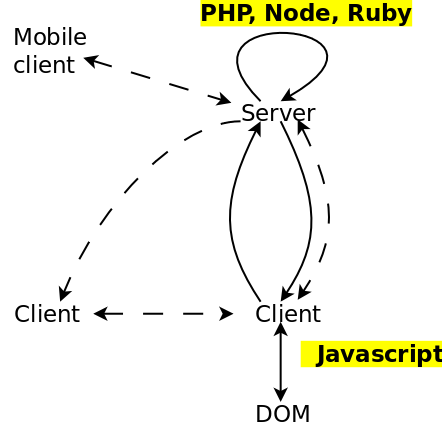
\includegraphics[width=0.7\textwidth]{web1.png}
\end{figure}
\end{frame}


\begin{frame}[fragile]{Бестиповость}

\begin{tabular}{l r}
  \begin{minipage}{5cm}
  \begin{block}{С сервера послали}
  \verb=1,0:Текст приветствия=
  \end{block}
  \begin{block}{На клиенте ожидалось}
  \verb=line <int>: <string>=
  \end{block}
  \end{minipage} & 
    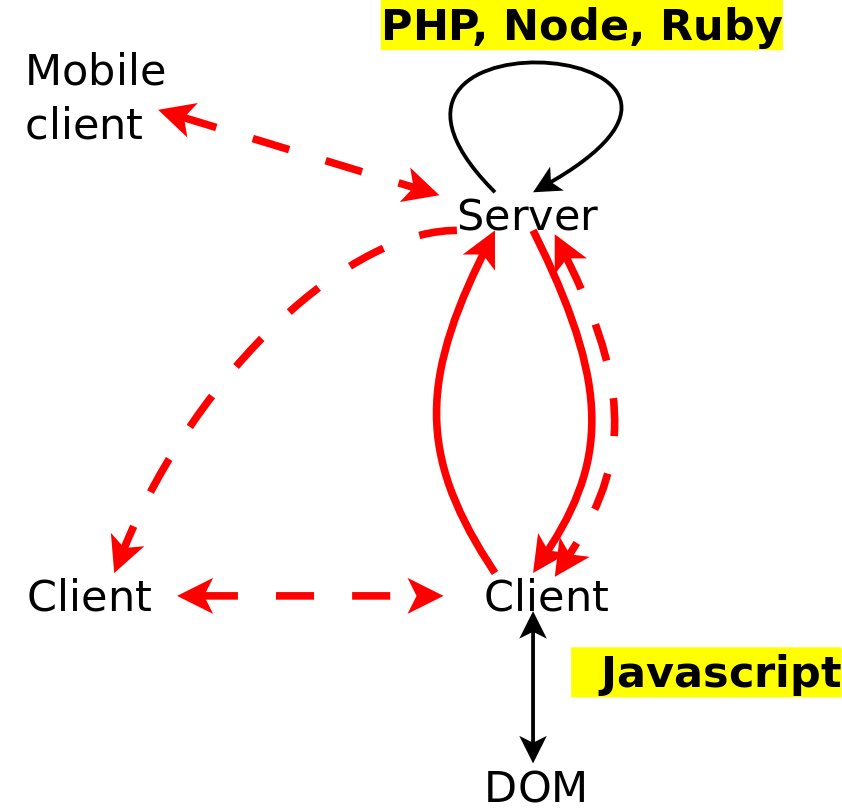
\includegraphics[width=.5\textwidth]{web2.png}
\end{tabular}   
\end{frame}


\begin{frame}{Хочется один tierless язык для всего}
\begin{center}

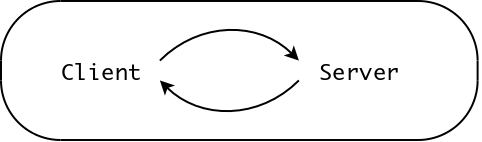
\includegraphics[width=0.8\textwidth]{ClientServer.png}
\vskip5mm
Другие tierless языки:\\
\vskip5mm
\begin{minipage}{0.34\textwidth}
\begin{itemize}
 \item Links
 \item Hop
 \item Ur/Web
 \item \textbf{Eliom}
\end{itemize}
\end{minipage}

\end{center}
\end{frame}

\begin{frame}[fragile]{}
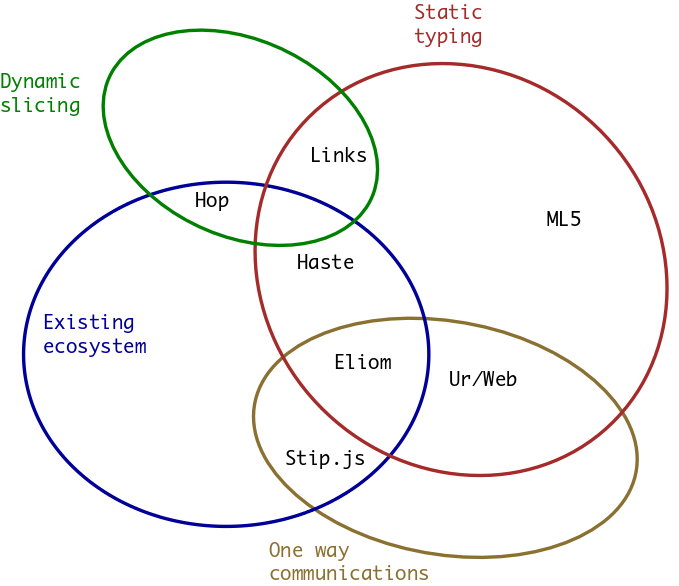
\includegraphics[width=.9\textwidth]{tierless.png}

Срисовано у \href{https://www.irif.fr/~gradanne/papers/talk_phdthesis.pdf#page=20}{Gabriel Radanne}
\end{frame}


\begin{frame}[fragile]
  
\includegraphics[width=.5\textwidth]{ocsigen.png}
  
\includegraphics[width=.4\textwidth]{INRIA_logo_2011.png}\\
  \vskip5mm
  \resizebox{\textwidth}{!}{
  \begin{tabular}{| l   l  |}
  \hline
  \multicolumn{2}{|c|}{\cellcolor{YellowGreen}Eliom} \\ \hline
  \cellcolor{Blueish}      Server & \cellcolor{yellow}Js\_of\_ocaml \\ \hline
  \multicolumn{2}{|c|}{OCaml} \\ \hline
  \end{tabular}
  }
\end{frame}

\begin{frame}[fragile]
  
\includegraphics[width=.5\textwidth]{ocsigen.png}\\
  \vskip5mm
  \resizebox{\textwidth}{!}{
  \begin{tabular}{| l   l  |}
  \hline
  \multicolumn{2}{|c|}{\cellcolor{YellowGreen}Library} \\ \hline
  \multicolumn{2}{|c|}{\cellcolor{YellowGreen}Syntax extension} \\ \hline

  \cellcolor{Blueish}      Server & \cellcolor{yellow}Js\_of\_ocaml \\ \hline
  \multicolumn{2}{|c|}{OCaml} \\ \hline
  \end{tabular}
  }
\end{frame}

\begin{frame}[fragile]{Серверная часть. Пример 1/2}
\begin{minted}{ocaml}
let service_with_params =
  Eliom_registration.Html.create
    ~path: ...
    ~meth:(Get ... )
    handler
\end{minted}
\pause\definecolor{links}{HTML}{2A1B81}
\hypersetup{colorlinks,linkcolor=,urlcolor=links}
\begin{itemize}
 \item Именованые параметры
 \item Можно больше одного сервиса на путь
 \item В данном случае из handler должен вернуться Html
\end{itemize}
% Если вместо числа пришло не число, то Eliom сам выдаст ошибку
\end{frame}

\begin{frame}[fragile]{Серверная часть. Пример 2/2}
\begin{minted}{ocaml}
let service_with_params =
  Eliom_registration.Html.create
    ~path:(Path ["horde"; "orc"])
    ~meth:(Get (int "i" ** (int "ii" ** string "s")))
    (fun (i,(ii,s)) -> 
       (* Тут обрабатываем Get запрос, 
          отдаём Html *)
    )
\end{minted}
\pause
\begin{itemize}
 \item Если параметр не подходит по типу -- ошибка
 \item Разумеется, пользовательские типы параметров поддержаны
 \item Нетипизированные параметры (список пар строк)
\end{itemize}

\end{frame}

\begin{frame}[fragile]{Порождение, например, Html}
\begin{minted}{ocaml}
Eliom_registration.Html.create ~path ~meth
  (fun _ ->
    let open Eliom_content.Html.D in
    let input = input ~a:[a_input_type `Text] () in
\end{minted}
\pause\vspace{-2pt}
\begin{minted}{ocaml}
    let button =
      button ~a:[a_onclick ...] [pcdata "Read value"]
    in
\end{minted}
\pause\vspace{-2pt}
\begin{minted}{ocaml}
    Lwt.return
         (html
            (head (title (pcdata "Test")) [])
            (body [input; button])))
  )
\end{minted}
\end{frame}

\begin{frame}[fragile]{Типизация через полиморфные варианты}
\begin{minted}{ocaml}
(* OK *)
script ~a:[a_async ()] (pcdata "http://something");  

(* ERROR *)
h2 ~a:[a_async ()] [pcdata "Some text"];
\end{minted}

Больше информации в 
\href{https://caml.inria.fr/pub/docs/manual-ocaml/lablexamples.html#sec46}{OCaml manual}

В Haskell их пытаются \href{https://hackage.haskell.org/package/data-diverse-2.0.1.0/docs/Data-Diverse-Which.html}
{эмулировать}, 
но выглядит страшно :)
% что есть не как в Elm, потому что их нет в явном виде даже в Haskell
\end{frame}

\begin{frame}[fragile]{Три семантики для создаваемых тегов}
DOM-семантика
\begin{minted}{ocaml}
    Eliom_content.Html.D
\end{minted}
``Функциональная``
\begin{minted}{ocaml}
    Eliom_content.Html.F
\end{minted}
Реактивная
\begin{minted}{ocaml}
    Eliom_content.Html.R
\end{minted}
\vskip5mm
Если нужно, то можно использовать все три одновременно
\end{frame}

\begin{frame}[fragile]{D. vs F.}
\begin{minted}{ocaml}
let b = button ~a:... [pcdata "text"] in
div [ b; b; b]
\end{minted}
\vskip5mm
По значению vs. по ссылке
\end{frame}

\begin{frame}[fragile]{Реактивность. Пример}
\begin{minted}{ocaml}
let value_signal,set_value = React.S.create "initial"
\end{minted}
\pause\vspace{-2pt}
\begin{minted}{ocaml}
let content_signal : _ React.signal =
  React.S.map (fun str ->
    let l = split str in
    let ps = l |> List.map 
      (fun s -> F.p [F.pcdata s]) in
    F.div ps
  )
  value_signal
\end{minted}
\pause\vspace{-2pt}
\begin{minted}{ocaml}
let make_client_nodes () =
  [ D.p [R.pcdata value_signal]
  ; R.node content_signal
  ]
\end{minted}
\end{frame}

\begin{frame}[fragile]{Про self-adjusting вычисления}
\verb=Incr_dom= от     \href{https://www.janestreet.com/}{Janestreet Capitals} \href{https://github.com/janestreet/incr_dom}{\faGithub}

\verb=Virtual DOM=  от \href{https://www.janestreet.com/}{Janestreet Capitals} \href{https://github.com/janestreet/virtual_dom}{\faGithub}

\verb=virtual-dom= от Matt-Esch \href{https://github.com/Matt-Esch/virtual-dom}{\faGithub} 
\vskip5mm
\href{https://blog.janestreet.com/self-adjusting-dom/}{Блогпост} из Janestreet Tech Blog
% иногда дорого заменять весь DOM по изменению сигнала. Тут на смену придут self-adjusting compuattions(SAC)
% Если их использовать, то будет перестраиваться только часть, та часть которая завязана на измененные данные.
\end{frame}

\begin{frame}[fragile]{Фрагменты клиентского и серверного кода}
\begin{minted}{ocaml}
let%server x  = ...

let%client y  = ...

let%shared z  = ...
\end{minted}
\vskip5mm
Всё в одном файле
\end{frame}

\begin{frame}[fragile]{Фрагменты клиентского кода на сервере}
\begin{minted}{ocaml}
let%server x = [%client 1 + 3 ]
\end{minted}

На клиенте считается \verb=1+3=.

Сервер оперирует этим как ''черным`` ящиком
\end{frame}

\begin{frame}[fragile]{Доступ к данным сервера на клиенте}
\begin{minted}{ocaml}
let%server s  : int = 1 + 2

let%client y  : int = ~%s + 1
\end{minted}
Ограничение -- jsonификация типа переменной s
\end{frame}

\begin{frame}[fragile]{Чуть более содержательный пример}
\begin{minted}{ocaml}
let%server counter action =
\end{minted}
\pause\vspace{-1em}
\begin{minted}{ocaml}
  let state = [%client ref 0 ] in
\end{minted}
\pause\vspace{-1em}
\begin{minted}{ocaml}
  button ~button_type:`Button
    ~a:[a_onclick [%client fun _ ->
\end{minted}
\pause\vspace{-1em}
\begin{minted}{ocaml}
          incr ~%state;
\end{minted}
\pause\vspace{-1em}
\begin{minted}{ocaml}
          ~%action !(~%state) 
       ]]
\end{minted}
\pause\vspace{-1em}
\begin{minted}{ocaml}
    [pcdata "Increment"]
\end{minted}
\end{frame}

\begin{frame}[fragile]{RPC}
\begin{minted}{ocaml}
let%server log str = (* тут логгируем str *)
\end{minted}
\pause\vspace{-2pt}
\begin{minted}{ocaml}
let%client log =
  ~%(Eliom_client.server_function 
      [%derive.json: string] 
      log)
\end{minted}
\pause\vspace{-2pt}
\begin{minted}{ocaml}
let%client () =
  Eliom_client.onload (fun () ->
    (* N.B. Серверные функции недоступны
       пока страничка не прогрузилась *)
    async (fun () -> 
      log "Hello from the client to the server!"))
\end{minted}
\end{frame}

\begin{frame}{Замечание про порядок вычислений}
Куски клиентского кода на сервере не вычисляются сразу.

Они регистрируются для последующего исполнения.

Когда страница прислана, то они начинают выполняться.
\end{frame}

\begin{frame}[fragile]{Объекты Javascript}
\pause
\begin{minted}{ocaml}
let options = object%js
  val         x = 3 (* read-only prop *)
  val mutable y = 4 (* read/write prop *)
end
\end{minted}
\end{frame}

\begin{frame}[fragile]{TyXML API vs. DOM API}
\begin{minted}{ocaml}
let n = div ~a:[a_id "some div id"]
  [ pcdata "aaa"
  ; pcdata "bbb" ]
let d = Eliom_content.Html.To_dom.of_div n
\end{minted}
\pause \vskip5mm \vskip10mm
\begin{minted}{ocaml}
let d =
  let d = createDiv document in  
  d##.id := (Js.string "some div id");
  appendChild d 
    (document##createTextNode (Js.string "aaa"));
  appendChild d 
    (document##createTextNode (Js.string "bbb"));
  d
\end{minted}
\end{frame}

% \begin{frame}[fragile]{}
% 1
% \end{frame}

\begin{frame}[fragile]{Компиляция OCaml кода}
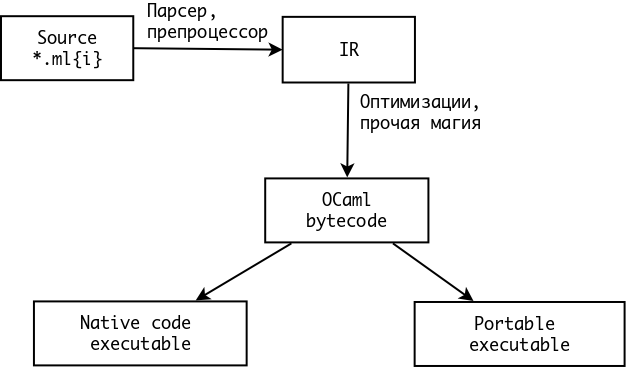
\includegraphics[width=1\textwidth]{compilation1.png}
\end{frame}

\begin{frame}[fragile]{Компиляция Eliom проекта}
\begin{center}
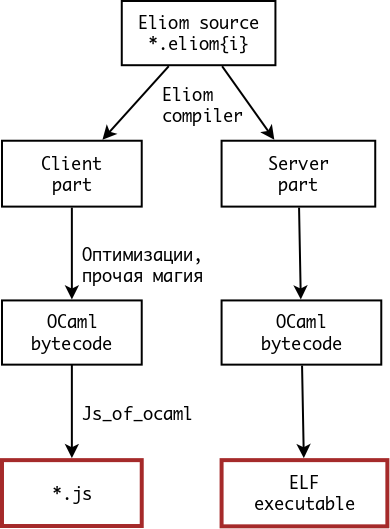
\includegraphics[width=0.5\textwidth]{compilation2.png}
\end{center}
\end{frame}

\begin{frame}[fragile]{Оптимизации $\rightarrow$ bytecode $\rightarrow$ Javascript}
\jsoo генерирует Javascript из \textbf{внутреннего} представления (bytecode)
\begin{itemize}
 \item[\faBad]  Получается нечитаемый код
 \item[\faBad]  Транслируется не очень быстро
 \pause
 \item[\faGood] Большинство фич языка можно использовать
 \item[\faGood] Больше оптимизаций, шустрее работает \href{https://www.irif.fr/~balat/publications/vouillon_balat-js_of_ocaml.pdf#page=13}
	  {\beamergotobutton{Графики тут}}
\end{itemize}
\vskip5mm
Следствие: всё что скомпилировалось в байткод, оттранслируется в Javascript

\pause
\vskip5mm
Elm \Huge \trollface

\end{frame}



\begin{frame}[fragile]{Ocsigen. Итоги}
\begin{itemize}
 \item ``Фишка'' -- tierless \pause
 \item Интеграция с существующим кодом на OCaml, \textbf{весь} синтаксис поддержан \pause
 \item Интеграция с существующим кодом на Javascript \pause
 \item Типобезопасность в целом \pause
 \item Можно оторвать \jsoo и использовать отдельно \pause
 \item[\faBad] Клиентская часть компилируется небыстро \pause
 \item[\faBad] Нечитаемый Javascript на выходе \pause
 \item[\faBad]  ``Адекватный'' синтаксис \pause
 \item[\faGood] ИМХО, адекватный
\end{itemize}

\end{frame}


\begin{frame}[fragile]{Другой вид трансляции}
Было:\\
*.ml $\xRightarrow{OCaml}$ bytecode $\xRightarrow{Js\!\_\!of\!\_\!ocaml}$ *.js
\vskip10mm\pause
А давайте теперь делать вот так:
*.ml $\Rightarrow$ *.js
\begin{itemize}
 \item Хотим уметь транслировать \textbf{весь} язык\pause
 \item [\faBad]  Все OCaml библиотеки надо перекомпилять 
 \item [\faBad]  Не были использованы OCaml-специфичные оптимизации
 \item [\faGood] Есть возможность сделать читаемый Javascript
 \item [\faGood] Быстрая (инкрементальная) трансляция
\end{itemize}
\vskip5mm\pause
Bucklescript от \href{https://www.techatbloomberg.com/}{Bloomberg}\\
\end{frame}

\begin{frame}[fragile]{Bucklescript\href{https://github.com/BuckleScript/bucklescript}{\faGithub}}
\href{https://bucklescript.github.io/bucklescript-playground/index.html}{Bucklescript песочница}
\vskip5mm
\pause
По сути backend к компилятору \vskip5mm\pause

Иногда, работает быстрее рукописного Javascript \vskip5mm\pause

\jsoo дружественнее к инфраструктуре OCaml, BuckleScript -- нет
\end{frame}

\begin{frame}[fragile]{Почти все проблемы решены...}
\faBad Кроме массового недовольства синтаксисом 
\vskip15mm \pause
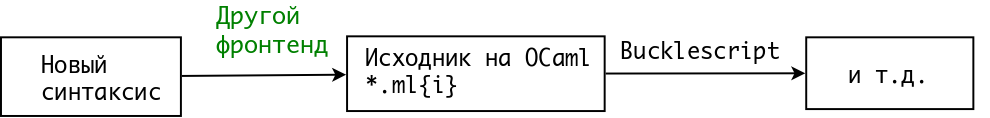
\includegraphics[width=.9\textwidth]{ReasonML.png}
\end{frame}

\begin{frame}[fragile]{ReasonML}
\href{https://reasonml.github.io/}{Сайт}
\vskip5mm
\href{https://reasonml.github.io/docs/en/comparison-to-ocaml.html}{Синтаксис Reason vs. OCaml}
\vskip5mm
\href{https://reasonml.github.io/en/try.html}{Песочница}
\vskip5mm
\href{https://www.reason-conf.com/}{ReasonConf} 11--13 мая 2018, Вена, Австрия
\end{frame}

\begin{frame}
\center{\Huge Вопросы?}
\end{frame}


\begin{frame}{Какие-то ссылки...}
 
Ocsigen demo \href{http://ocsigen.org/ocsigen-start/demo}{\faGithub} и
\href{http://ocsigen.org/ocsigen-start/demo/}{online}

Ocsigen \href{http://ocsigen.org/graffiti/}{graffiti} demo \href{https://github.com/ocsigen/graffiti}{\faGithub}
\end{frame}

\end{document}
